\section{Descripción Arquitectónica}
\hspace{1.27cm} El diagrama de bloques, la descripción de cada señal, y el diseño por medio de máquinas de estado del módulo \code{behavioral\_parkingController} correspondiente a la descripción estructural del controlador automatizado para la entrada de un estacionamiento se encuentran el informe correspondiente a la Tarea \#1, disponible en el \hyperref[git]{repositorio de GitHub}. La estructura de archivos que se utilizó para el código fuente de esta tarea es la siguiente:

\dirtree{%
.1 ./t2.
.2 Makefile.
.2 hdl.
.3 behavioral\_parkingController.v.
.2 include.
.3 state\_defs.vh.
.2 sim.
.3 testbench.v.
.3 tester.v.
.3 wave\_names.tff.
.3 waves.gtkw.
.2 synth.
.3 cmos\_cells.lib.
.3 cmos\_cells.v.
.3 cmos\_delay\_cells.v.
.3 cmos\_delay\_synth.ys.
.3 cmos\_synth.ys.
.3 rtlil\_synth.ys.
}

A continuación, se describe cada uno de estos archivos:
\begin{itemize}
    \item \code{Makefile}: Archivo para compilar código fuente y generar las simulaciones de forma automática.
    \item \code{behavioral\_parkingController.v}: Código conductual para el controlador de automatizado para la entrada de un estacionamiento desarrollado en la Tarea\#1. 
    \item \code{state\_defs.vh}: Archivo de encabezado que contiene las definciones de los estados para la máquina de estados en \code{behavioral\_parkingController.v}.
    \item \code{testbench.v}: Banco de pruebas para las simulaciones.
    \item \code{tester.v}: Probador para generar los vectores de prueba correspondiente al plan de pruebas.
    \item \code{wave\_names.tff}: `Transfer Filter File'. Utilizado para reemplazar las codificaciones de los estados por sus nombres en \code{state\_defs.vh} en \code{gtkwave}.
    \item \code{waves.gtkw}: Contiene la configuración de inicio de \code{gtkwave}. 
    \item \code{cmos\_cells.lib}: Librería de compuertas estándar proporcionada por el profesor.
    \item \code{cmos\_cells.v}: Descripción conductual de las compuertas contenidas en \code{cmos\_cells.lib}
    \item \code{cmos\_delay\_cells.v}: Descripción conductual de las compuertas contenidas en \code{cmos\_cells.lib}, con retardos.
    \item \code{cmos\_synth.ys}: Script de Yosys para sintetizar el módulo \code{behavioral\_parkingController} utilizando \code{cmos\_cells.lib} 
    \item \code{cmos\_delay\_synth.ys}: Script de Yosys para sintetizar el módulo \code{behavioral\_parkingController.v} utilizando \code{cmos\_cells.lib} con retardos. 
    \item \code{rtlil\_synth.ys}: Script de Yosys para sintetizar el módulo \code{behavioral\_parkingController} utilizando \code{RTLIL} para crear una descripción estructural genérica. 
\end{itemize}
En las siguientes secciones, se especificará como se abordó la síntesis del módulo conductual por medio de las librerías \code{RTLIL} y \code{cmos\_cells.lib}.

\subsection{Cambios con respecto al diseño de la Tarea \#1}
Para lograr que el módulo \code{behavioral\_parkingController} sintetizara correctamente para ambas librerías utilizadas, se tuvieron que realizar dos cambios importantes:
\begin{itemize}
    \item \textbf{Uso de parámetros en la declaración del módulo}: En la primera tarea, se proporcionaba al módulo con el parámetro \code{correct\_code} correspondiente a los últimos 4 dígitos del carnet del estudiante al declarar el módulo en el banco de pruebas. Como Yosys solo recibe el archivo que contiene el módulo y no toma en cuenta las declaraciones para la síntesis, este tipo de parámetros no son sintetizados correctamente con la herramienta. Por tanto, \code{correct\_code} se declaró como \code{localparam} dentro del módulo, y se quitó la opción de pasarle el parámetro \code{correct\_code} al módulo a la hora de declararlo. 
    \item \textbf{Variables inicializadas ante un reset}: En el bloque \code{always} correspondiente a la transición de estados, se incluyeron líneas adicionales para inicializar las salidas del módulo. Sin embargo, esto no es necesario, ya que la inicialización de las salidas la realiza la lógicombinacional del módulo y no la secuencial. Por tanto, esto se removió del módulo. 
\end{itemize}

\subsection{Problemas encontrados}
Después de hacer los cambios mencionados en la sección anterior, aún se encontraron problemas en la síntesis que no pudieron ser resueltos. 
El problema que se encontró está relacionado a la síntesis con \code{RTLIL}. 
A pesar de que en la lógica combinacional del módulo se definió el valor por defecto de \code{next\_state} y \code{next\_attempt} como \code{state} y \code{attempt} respectivamente, este no fue el comportamiento que se observaba en las formas de onda. El comportamiento de \code{state}, \code{attempt}, y las salidas del módulo son las correctas, pero las variables mencionadas inicialmente se mostraban como condición no importa en la forma de onda, hasta que llegaran los estímulos necesarios para que \code{state} o \code{attempt} cambiaran. Esto difiera del comportamiento del módulo conducutal de la Tarea \ 1, ya que estas condiciones no importa no se presentaron en su momento.

\begin{figure}[!h]
    \centering
    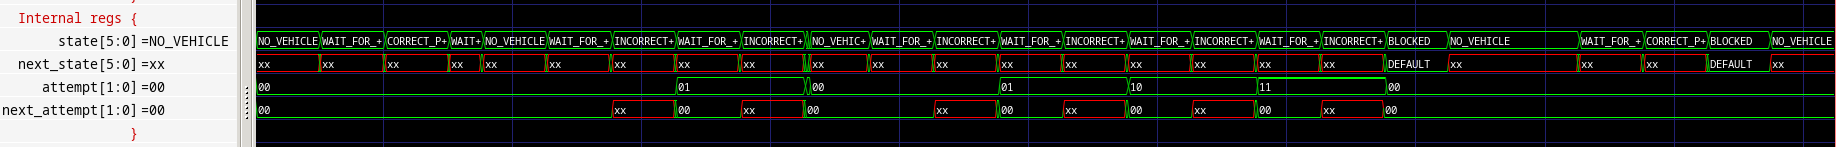
\includegraphics[width = \linewidth]{figs/inusual.png}
    \caption{Comportamiento inusual en las variables próximas al realizar la síntesis con \code{RTLIL}}
    \label{inusual}
\end{figure}


Este problema no se presentó en la síntesis con \code{cmos\_cells.lib}. 
Se cree que esto es causado por la forma en que \code{RTLIL} maneja los flip-flops. 

\newpage 

\subsection{RTLIL}
Para realizar la síntesis por medio de \code{RTLIL}, se utilizó el siguiente script de Yosys:

\begin{minted}[bgcolor=lightgray]{bash}
read_verilog -I./include ./hdl/behavioral_parkingController.v
hierarchy -check -top behavioral_parkingController
proc; opt; fsm; opt; memory; opt
techmap; opt
clean
write_verilog synth/rtlil_synth_parkingController.v
\end{minted}

La síntesis por medio de esta librería da como resultado multiplexores, ALUs, LUTs, etc. ya que depende de la librería interna de Yosys.

\subsection{cmos\_cells.lib}
Para realizar la síntesis por medio de \code{cmos\_cells.lib}, se utilizó el siguiente script de Yosys:

\begin{minted}[bgcolor=lightgray]{bash}
read_verilog -I./include ./hdl/behavioral_parkingController.v
hierarchy -check -top behavioral_parkingController
proc; opt; fsm; opt; memory; opt
techmap; opt
dfflibmap -liberty ./synth/cmos_cells.lib
abc -liberty ./synth/cmos_cells.lib
clean
write_verilog ./synth/cmos_synth_parkingController.v
\end{minted}
La siguiente tabla indica la cantidad de compuertas resultantes de la síntesis:

\begin{figure}[!h]
    \centering
    \begin{tabular}{cc}
        \toprule
        \textbf{Tipo e compuerta} & \textbf{Cantidad} \\
        \midrule
        NAND    & 41 \\
        NOR     & 48 \\
        NOT     & 21 \\
        FF-D    & 8 \\
        \bottomrule
    \end{tabular}
    \caption{Número de componentes resultantes de la síntesis utilizando \code{cmos\_cells.lib}}
\end{figure}
\subsection{Simulación con retardos}
Para la síntesis utilizando compuertas que tienen retardos, se modificó el archivo \code{cmos\_cells.v} y se le agregó un retardo de una unidad de tiempo al flip-flop D, tal que:

\begin{minted}[bgcolor=lightgray]{verilog}
always @(posedge C) Q <= #1 D;
\end{minted}

De esta manera, se realizó una simulación que tome en cuenta retardos en la respueta de las celdas de \code{cmos\_cels.lib}.
En secciones posteriores, se calculará este tiempo de propagación por medio de las formas de onda de \code{gtkwave}.
El archivo de síntesis que se desarrolló para este caso es muy similar al utilizado con \code{cmos\_cells.lib}, con la diferencia que se utilizó un archivo diferente de escriptura para el código estructural de Verilog, con el propósito de que las 3 simulaciones puedan ser ejecutadas con un solo comando.
